\documentclass{llncs}
\usepackage{fullpage}

%load needed packages
\usepackage{graphicx}
\usepackage{array}
\usepackage{booktabs}
\usepackage[utf8]{inputenc}
\usepackage{amsmath} 
\usepackage{hyperref}


\begin{document}

\title{Task B}
\subtitle{Supervised Learning Model Evaluation Metrics}

\author{Diego De Pablo}
\institute{\email{depablodiego@uma.es} \\
Health Engineering. Málaga University.}

\maketitle 

\vspace{1cm} % Space down the title

\textit{
	This work investigates the performance of various classification methods in a supervised learning context, focusing on how certain techniques can yield misleadingly high metrics. Specifically, some methods that classify all samples into a single category may achieve better performance metrics compared to methods that accurately differentiate between positive and negative samples. The analysis highlights the importance of robust metrics like the Jaccard index and F-measure, which provide valuable insights into model performance. Ultimately, it underscores the necessity of understanding the specific goals of the analysis to determine which metrics are most relevant for evaluating a model’s effectiveness. }



\section{Introduction}

Artificial intelligence (AI) has emerged as a transformative solution to numerous challenges in a wide range of domains, often being viewed as a key to simple and efficient problem-solving. However, the performance of AI models must be critically assessed to understand their real-world applicability and limitations. In particular, supervised learning algorithms are often used in classification tasks, where the performance of these models can be evaluated through specific metrics.


\section{Dataset Description}

The aim of this work is to highlight the validation methods and explore examples ranging from realistic to exaggerated cases that, in certain scenarios, might be considered good results if certain metrics are ignored. Even though these results may seem favorable, they can actually be misleading. To demonstrate this, we will base our analysis on the following dataset (observe the figure \ref{fig:dataset}).

\begin{figure}[h!]
	\begin{center}  % Usamos el entorno 'center'
		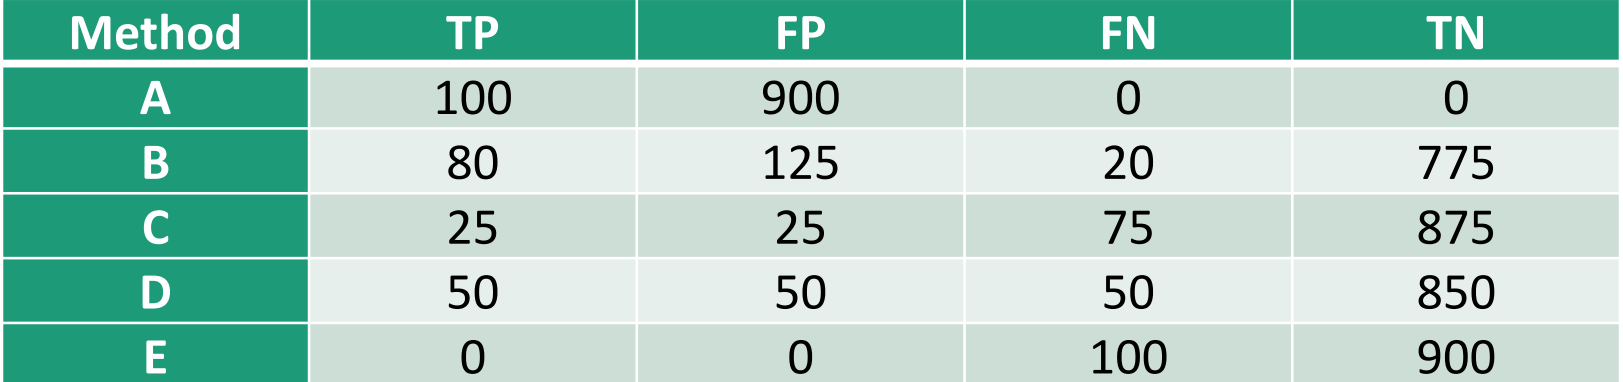
\includegraphics[width=1\textwidth]{images/dataset.png}
		\caption{The methods studied in this work}
		\label{fig:dataset}
	\end{center}
\end{figure}

\vspace{-20pt} % Ajusta este valor para reducir el espacio



\section{Conclusion}


\section{Repository Github}
Further information, including the source code and full project documentation, can be accessed through the GitHub repository.  \href{https://github.com/Diegodepab/Supervised_Learning_Model_Evaluation_Metrics}{Click here to go to the repository.} 



\bibliographystyle{plain}  % Puedes cambiar "plain" por el estilo de tu preferencia, como apalike, ieeetr, etc.
\bibliography{bibliography}  % Aquí va el nombre de tu archivo .bib (sin la extensión .bib)
\end{document}
